\documentclass[12pt]{article}
\usepackage[spanish,mexico]{babel}
	\selectlanguage{spanish}
\usepackage{graphicx}
\usepackage{amsmath}
\usepackage{wrapfig}
\usepackage{float}
\usepackage[utf8]{inputenc}

\usepackage{graphicx}
\graphicspath{{images/}}

%\usepackage{vmargin}
%\setmarginsrb{3 cm}{2.5 cm}{3 cm}{2.5 cm}{1 cm}{1.5 cm}{1 cm}{1.5 cm}

\title{Actividad 3: Interpolación de datos}
\author{Martín Alejandro Paredes Sosa}
\date{Febrero 2016}

\begin{document}

\maketitle

\section{Introducción}

En el campo del análisis numérico, la interpolación es un método para construir nuevos puntos de información dentro de una secuencia de datos conocidos. \\
En el campo de de la ciencia e ingeniería, estos datos se obtienen mediante experimentación y muestreo, los cuales representan los valores de una función para un limitado numero de valores de la variable independiente. Estos usualmente se requiere estimar el valor de la función para un valor intermedio de la variable independiente.\cite{wikiI}

\section{Actividad}

En esta actividad aprenderemos un poco del proceso de encontrar una función que interpole todos los puntos, apoyados en la función scipy.interpolate de Python.\cite{a} \\

El scipy.interpolate es un sub-paquete que contiene funciones y clases spline, interpolación unidimensional y multi-dimensional, Lagrange y Taylor interpoladores polinómicas y contenedores para la funciones FitPack y DFITPACK.\cite{scipy} \\

Para esta actividad se utilizo interp1d, el cual interpola una función 1-D. Esta función toma valores $x$ y $y$, los cuales son matrices, los cuales son utilizados para aproximarse a alguna función f: y= f(x).\cite{In1D}
\pagebreak

La actividad a realizar esta basada en el siguiente código ejemplo:

\subparagraph{Código Ejemplo} 

\begin{verbatim}
import numpy as np
import matplotlib.pyplot as plt
from scipy.interpolate import interp1d

# Original "data set" --- 21 random numbers between 0 and 1.
x0 = np.linspace(-1,1,21)
y0 = np.random.random(21)

plt.plot(x0, y0, 'o', label='Data')

# Array with points in between those of the data set for interpolation.
x = np.linspace(-1,1,101)

# Available options for interp1d
options = ('linear', 'nearest', 'zero', 'slinear', 'quadratic', 'cubic', 10)

for o in options:
    f = interp1d(x0, y0, kind=o)    # interpolation function
    plt.plot(x, f(x), label=o)      # plot of interpolated data

plt.legend()
plt.show()
\end{verbatim}

\begin{figure}[H]
	\centering
	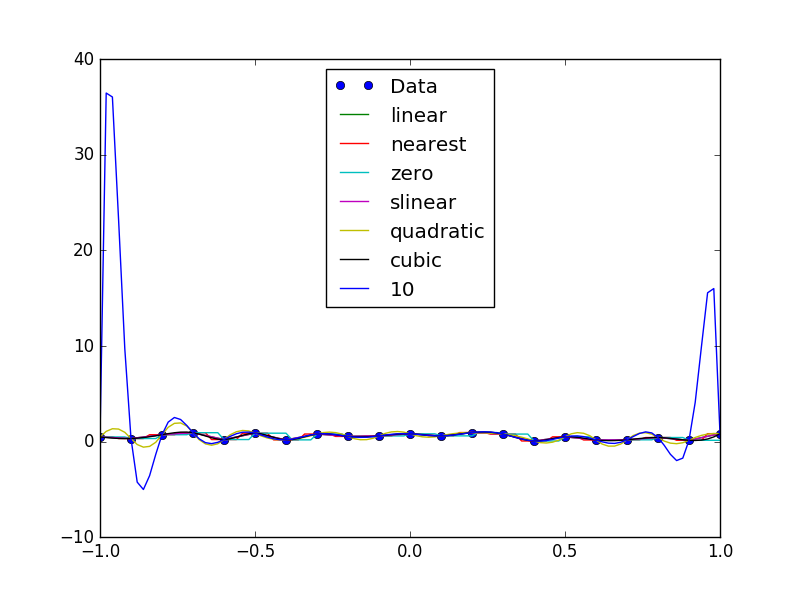
\includegraphics[width=7.5cm, height=4.5cm]{CodigoBase.png}
	\caption{Resultado del código original}
\end{figure}

\section{Resultados}

Los ejercicios de esta actividad nos pide realizar una interpolación lineal, cuadrática y  cúbica de una serie de datos generados de manera aleatoria dentro de un rango y en base a una función. \cite{a}

\subparagraph{10 puntos aleatorios entre x=[0,3] para la función f(x)= $\sin(2x)$}
\begin{verbatim}
import numpy as np
import matplotlib.pyplot as plt
from scipy.interpolate import interp1d

#Generando datos
x01 = np.random.random(10)
x1 = 3.0*x01
y1 = np.sin(2.0*x1)

#Graficar los puntos aleatorios x y los f(x)=Sin(2x)
plt.plot(x1, y1, 'o', label='Data')

#Punto para interpolar
x = np.linspace(min(x1),max(x1),101)

#Opciones para interp1d
opc = ('linear', 'quadratic', 'cubic')

for o in opc:
    f = interp1d(x1, y1, kind=o)
    plt.plot(x, f(x), label=o)

#Mostrar la grafica
plt.legend(loc='best')
plt.show()
\end{verbatim}
\pagebreak
Resultado:
\begin{figure}[H]
	\centering
	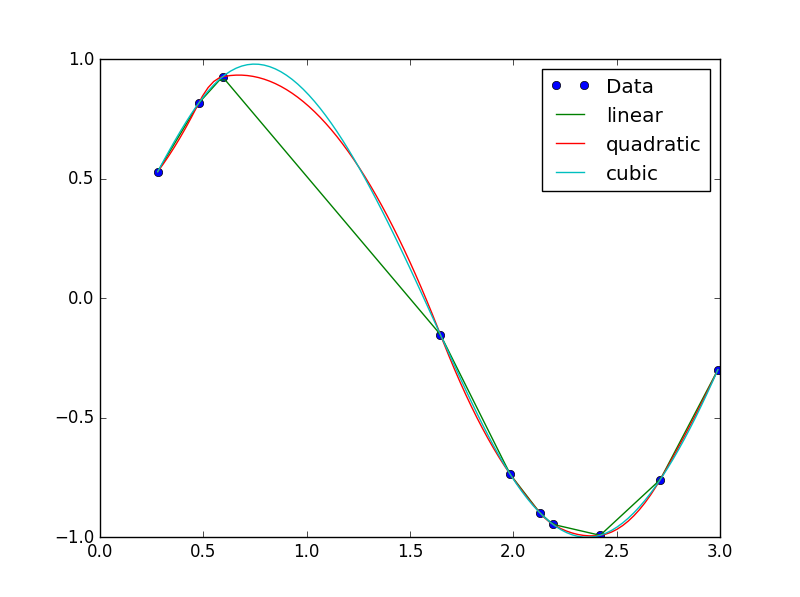
\includegraphics[width=7.5cm]{Sin2x.png}
	\caption{Resultado para la interpolación de f(x)= $\sin(2x)$}
\end{figure}

\subparagraph{20 puntos aleatorios entre x=[-10,10] para la función f(x)= $\sin(x)/x$}
\begin{verbatim}
import numpy as np
import matplotlib.pyplot as plt
from scipy.interpolate import interp1d

#Generando datos
x01 = np.random.random(20)
x1 = 20.0*x01-10.0
y1 = (np.sin(x1))/x1

#Graficar los puntos aleatorios x y los f(x)=Sin(2x)
plt.plot(x1, y1, 'o', label='Data')

#Punto para interpolar
x = np.linspace(min(x1),max(x1),200)

#Opciones para interp1d
opc = ('linear', 'quadratic', 'cubic')

for o in opc:
    f = interp1d(x1, y1, kind=o)
    plt.plot(x, f(x), label=o)

#Mostrar la grafica
plt.legend(loc='best')
plt.show()
\end{verbatim}
Resultado:
\begin{figure}[H]
	\centering
	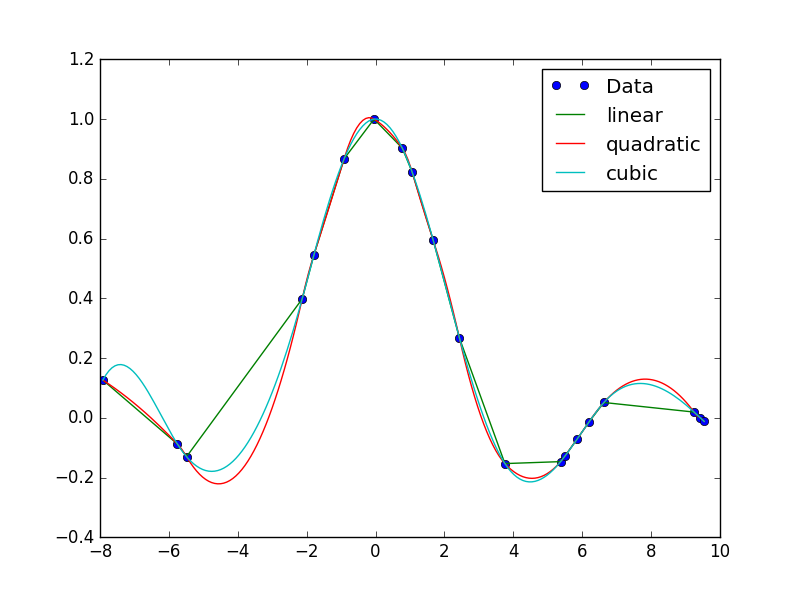
\includegraphics[width=7.5cm]{SinXentreX.png}
	\caption{Resultado para la interpolación de f(x)= $\sin(x)/x$}
\end{figure}

\subparagraph{16 puntos aleatorios entre x=[-3,3] para la función f(x)= $x^2 \sin(2x)$}
\begin{verbatim}
import numpy as np
import matplotlib.pyplot as plt
from scipy.interpolate import interp1d

#Generando datos
x01 = np.random.random(16)
x1 = 6.0*x01-3.0
y1 = (x1*x1)*(np.sin(2.0*x1))


#Graficar los puntos aleatorios x y los f(x)=Sin(2x)
plt.plot(x1, y1, 'o', label='Data')

#Punto para interpolar
x = np.linspace(min(x1),max(x1),200)

#Opciones para interp1d
opc = ('linear', 'quadratic', 'cubic')

for o in opc:
    f = interp1d(x1, y1, kind=o)
    plt.plot(x, f(x), label=o)

#Mostrar la grafica
plt.legend(loc='best')
plt.show()
\end{verbatim}
Resultado:
\begin{figure}[H]
	\centering
	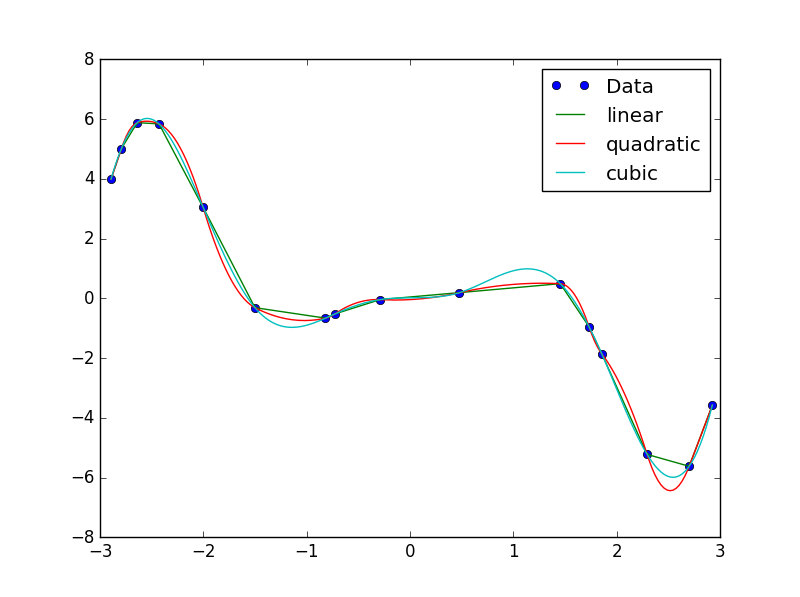
\includegraphics[width=7.5cm]{x2Sin2x.png}
	\caption{Resultado para la interpolación de f(x)= $x^2 \sin(2x)$}
\end{figure}


\subparagraph{12 puntos aleatorios entre x=[-2,2] para la función f(x)= $x^3 \sin(3x)$}
\begin{verbatim}
import numpy as np
import matplotlib.pyplot as plt
from scipy.interpolate import interp1d

#Generando datos
x01 = np.random.random(12)
x1 = 4.0*x01-2.0
y1 = (x1*x1*x1)*(np.sin(3.0*x1))


#Graficar los puntos aleatorios x y los f(x)=Sin(2x)
plt.plot(x1, y1, 'o', label='Data')

#Punto para interpolar
x = np.linspace(min(x1),max(x1),200)

#Opciones para interp1d
opc = ('linear', 'quadratic', 'cubic')

for o in opc:
    f = interp1d(x1, y1, kind=o)
    plt.plot(x, f(x), label=o)

#Mostrar la grafica
plt.legend(loc='best')
plt.show()
\end{verbatim}
Resultado:
\begin{figure}[H]
	\centering
	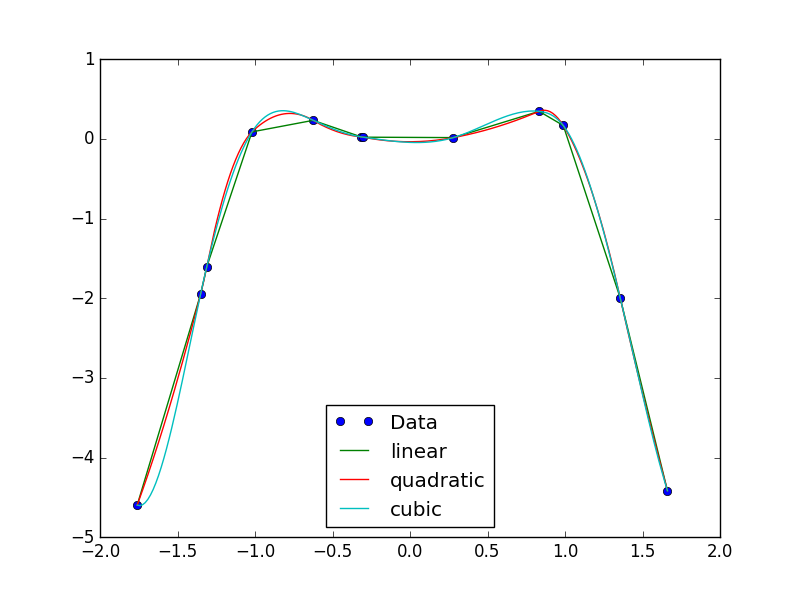
\includegraphics[width=7.5cm]{x3_Sin3x.png}
	\caption{Resultado para la interpolación de f(x)= $x^3 \sin(3x)$}
\end{figure}


\begin{thebibliography}{6}
	
	\bibitem{wikiI}
	Wikipedia (2016)
	\textit{Interpolation}. Recuperado de:\\ https://en.wikipedia.org/wiki/Interpolation
	
	\bibitem{a}
	Lizárraga, C. (2016)
	\textit{Actividad 3 (2016-1)}. Recuperado de: http://computacional1.pbworks.com/w/page/104792695/Actividad\%203\%20(2016-1)	
	
	\bibitem{scipy}	
	ENTHOUGHT (2016)
	\textit{Interpolation (scipy.interpolate)} Recuperado de:\\ http://docs.scipy.org/doc/scipy/reference/interpolate.html\#module-scipy.interpolate
	
	\bibitem{In1D}	
	ENTHOUGHT (2016)
	\textit{scipy.interpolate.interp1d} Recuperado de:\\ http://docs.scipy.org/doc/scipy/reference/generated/scipy.interpolate.interp1d.html\# scipy.interpolate.interp1d


\end{thebibliography}


\end{document}